
\chapter{Conceito de IoT no cultivo da Salicórnia}

A palavra salicórnia deriva do latim tardio \textit{sal}, que significa sal, e \textit{cornus} que significa corno. Etimologicamente a palavra salicórnia significa cornos salgados\cite{chambers}. A espécie de salicórnia que que servirá de mote à elaboração desta dissertação é a única existente em Portugal designada por \sr \textit{J. Woods (S. ramosissima)}\cite{JoaoSilva}, uma espécie do género \textit{Salicornia L.}, pertencente à família das beterrabas denominada de \textit{Chenopodiaceae} \cite{chenopodiaceae}.

Nesta secção será apresentada a \sr que impulsionará toda esta dissertação. Serão descritas as principais características desta planta, principais propriedades e as diferentes aplicações alimentais existentes no mercado. 

\section{Características da planta}


A salicórnia é uma espécie halófita, ou seja adaptada a viver em ambientes com elevado teor salino\cite{ferri}, sendo uma das mais evoluídas da sua família. É uma planta anual de dimensão pequena, aparentemente sem folhas, ereta, os seus caules são carnudos e suculentos, simples e/ou extremamente ramificados, segmentados por articulações\cite{Silva2000}, geralmente com menos de 30 cm de altura\cite{overviewsal}.

A salicórnia tem uma coloração normalmente verde-escuro mas a sua ramagem torna-se  verde-amarelado ou mesmo vermelho-púrpura no outono\cite{Silva2000}. A figura \ref{primoutono} ilustra a respetiva coloração na primavera e no outono. Na Inglaterra, a salicórnia é conhecida como \textit{purple glasswort}, podendo este nome estar na origem desta pigmentação caraterística\cite{Davy2001}. Em Portugal e Espanha é conhecida vulgarmente como erva-salada, sal verde e/ou espargos do mar\cite{RaquelPinto}. 

\newpage
\begin{figure}[!htb]
	\centering
	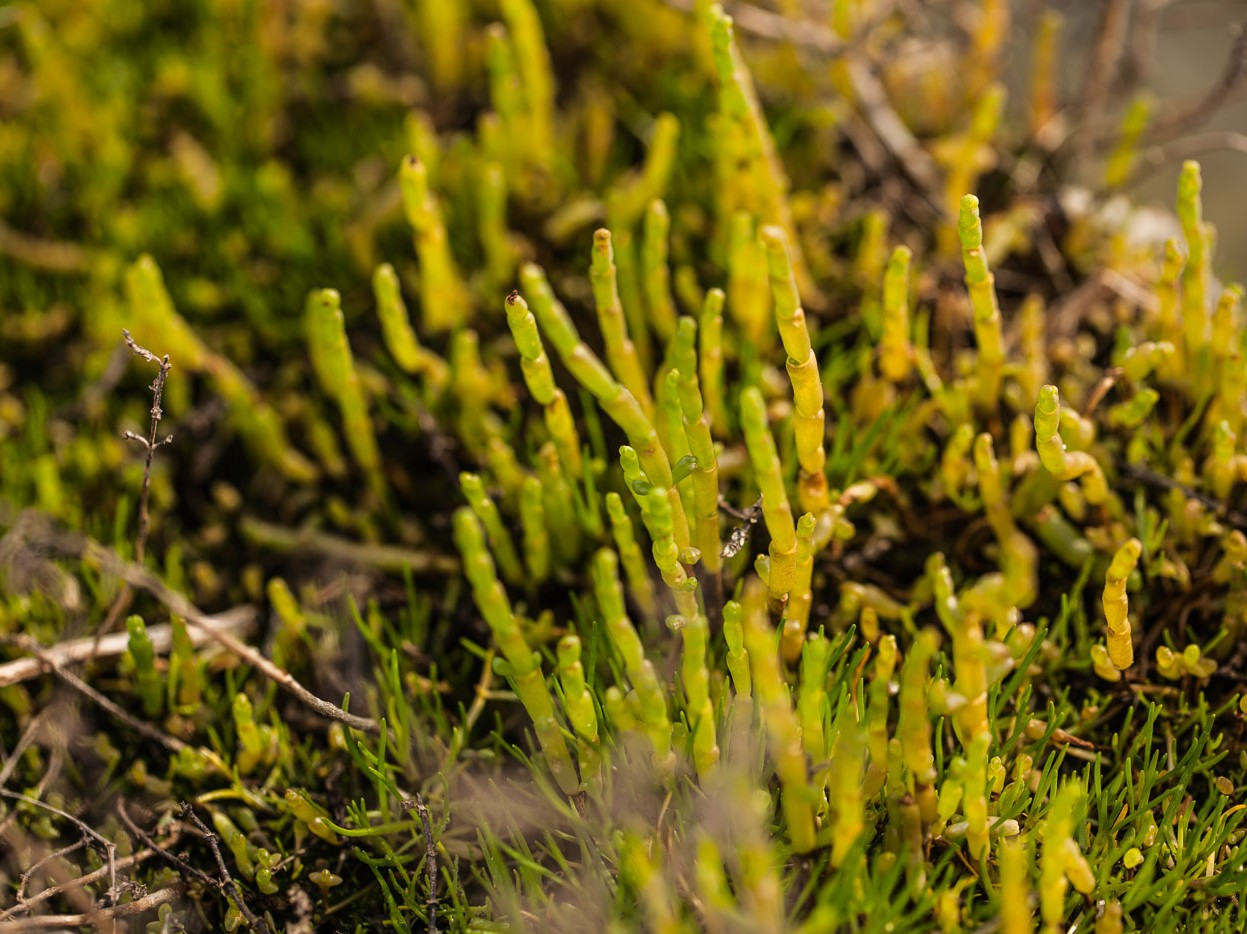
\includegraphics[scale=0.3]{img/cap2-sali/Salicornia04.JPG}
	\caption{\sr: na primavera e no outono respetivamente à esquerda e à direita (Fotografia por José M. G. Pereira)}
	\label{primoutono}
\end{figure}


A \sr desenvolve-se preferencialmente no litoral costeiro, em pântanos e sapais salgados ou em margens de salinas temporariamente alagadas. Encontra-se distribuída maioritariamente na parte oeste da Europa e a oeste da região do Mediterrâneo, sendo uma das espécies mais abundante\cite{Figueroa1987}. Pode ser encontrada em todo o litoral da Península Ibérica, embora com menos frequência no Minho\cite{Silva2000}. Em Portugal, é encontrada ao longo da costa, mais frequentemente nas margens dos canais da Ria de Aveiro e Ria Formosa, no Algarve\cite{RaquelPinto}. 

Esta planta é uma das mais estudadas a nível mundial\cite{Figueroa1987}, possuindo um ciclo de vida anual bem definido, com gerações discretas e as suas sementes são hermafroditas\cite{Silva2007}. A salicórnia cresce habitualmente entre março, início da sementeira e novembro fechando assim o ciclo com a produção de sementes. Entre maio  e agosto decorre a colheita da planta\cite{RaquelPinto} utilizada para os mais diversos fins. A floração ocorre fundamentalmente no mês de outubro\cite{Figueroa1987}. A figura \ref{ciclodevida} representa evolução do estado da planta para as diferentes fases do seu ciclo de vida. 




 \begin{figure}[!htb]
 	\centering
 	
\includegraphics{uaLogoNew.pdf}
 	\caption{Ciclo de vida da \sr (Fotografia por José M. G. Pereira)}
 	\label{ciclodevida}
 \end{figure}
 
 



\newpage

\section{Importância da planta}


Uma das características que tornam o género \textit{Salicornia L} uma planta tão popular são as suas elevadas propriedades nutricionais, nomeadamente a nível de minerais e vitaminas antioxidantes, como vitamina C e $\beta$-caroteno. A salicornia é também uma fonte de proteínas e possui um alto teor total de lípidos e ómega-3[ref].   %(Ventura et al., 2011a)


Desde a descoberta da salicórnia que esta é usada a nível culinário mas também no tratamento e prevenção de algumas doenças. Seguidamente iremos aprofundar cada uma dessas aplicações esclarecendo a sua relevância. 



\subsection{Aplicações alimentares}


Espécies do género \textit{Salicornia L.} estão incluídas na alimentação humana, desde a antiguidade, sendo normalmente consumida crua, cozinhada ou seca, podendo ser triturada. Quando crua é usada como acompanhamento das mais diversas refeições enquanto que seca ou triturada é usada como especiaria, podendo ser utilizada como tempero na confeção de peixes, marisco ou carnes. O sal verde é um grande substituto do sal comum, pois é rico em substâncias depurativas e diuréticas. Os seus caules carnudos são bastante requisitados para cozinhas \textit{gourmet}, não só pelo seu sabor salgado, mas também pelo seu elevado valor nutricional.  [reff]


 

%especifiaria, conhecida como sal verde, podendo ser utilizado maioritariamente para tempero 

%A Salicórnia seca e triturada, transforma-se numa especiaria – Sal Verde – podendo ser utilizada como tempero. O Sal Verde é mais vantajoso em relação ao sal comum, pois é rico em substâncias depurativas e diuréticas (Raposo et al., 2009).

%A Salicórnia pode ser consumida crua ou cozinhada. Crua, pode acompanhar saladas ou batatas. Em conserva de vinagre pode acrescentar uma nota ácida a diversos pratos. Cozida em água durante cerca de 10 minutos pode depois ser salteada em manteiga.


%Associada com frequência na confeção de peixe e marisco, conceituados chefs internacionais introduzem-na em pratos de carne, nomeadamente borrego.


\subsection{Aplicações medicinais}


A nível medicinal, existem inúmeros estudos que revelam as propriedades químicas que esta planta detém. Existem estudos que demonstram estas propriedades na prevenção e tratamento de algumas doenças, tais como, a hipertensão, cefaleias e escorbuto, diabetes, obesidade, cancro, entre outras.


\section{Condições ideais de cultivo da salicórnia}

O crescimento da \sr é influenciada pela salinidade do meio. Um estudo realizado por Silva et al.\cite{Silva2007} comprova que esta planta halófita apresenta um crescimento ideal a salinidades baixas ou moderadas, em vez de salinidades elevadas, pelo que é considerada uma halófita não obrigatória.


%alterar bastante o texto... palha









Nesta secção encontra-se descrita uma pequena introdução ao conceito de \textit{Internet of Things} e respetiva importância no contexto deste projeto. São também apresentadas as principais tecnologias de comunicação possível de utilização e respetiva comparação entre elas. Por fim, serão apresentados alguns projetos/aplicações relacionadas com esta dissertação.  


%a \sr que impulsionará toda esta dissertação. Serão descritas as principais características desta planta, principais propriedades e as diferentes aplicações alimentais existentes no mercado. 



\section{Evolução tecnológica: o IoT}


Antes de descrever a importância e o conceito de \ac{IoT}, é necessário entender as diferenças entre os termos Internet e\ac{WWW}, que 	são usados indistintamente pela sociedade. A Internet é a camada ou rede física composta por \textit{switches}, \textit{routers} e outros equipamentos\cite{Evans2011a}. A sua principal função é transportar informações de um ponto para outro de forma rápida, confiável e segura. Por outro lado, a Web pertence à camada de aplicações que opera sobre a Internet cuja função é oferecer uma interface que transforme as informações que fluem pela Internet em algo útil. Ao longo do tempo, a Web passou e continua a passar por várias etapas evolucionárias, identificadas como:

\begin{itemize}
	\item \textbf{Web 1.0 - passado}: esta primeira etapa foi inventada por Tim Berners Lee em 1989\cite{Getting}. Nesta fase surgiram os principais conceitos que conhecemos da Internet atual: Localizador Uniforme de Recursos (do inglês \ac{URL}), Linguagem de Marcação de Hipertexto (do inglês \ac{HTML}) e Protocolo de Transferência de Hipertexto (do inglês \ac{HTTP}). Ainda nesta primeira fase, mas mais tarde, em 1998 foi criado por Larry Page e Sergey Brin o Google que criou simplicidade nas pesquisas na Web\cite{Lovato2014}. 
	
	\item \textbf{Web 2.0 - presente}: a Web cresceu muito e muito rapidamente. A versão mais próxima da visão de Tim Berners Lee – colaborativa, usado como meio de interação, comunicação global e elevado compartilhamento de informação. 
	
	\item \textbf{Web 3.0 - futuro}: para o futuro prevê-se que os conteúdos online possão vir a estar organizados de forma semântica, muito mais personalizados para cada utilizador, sites, aplicações inteligentes e/ou publicidade baseada nas pesquisas e nos comportamentos.
\end{itemize}

O aparecimento do IoT foi extraordinariamente importante já que se trata da primeira evolução real da Internet, um salto que levará, no futuro, ao desenvolvimento de aplicações revolucionárias com potencial para melhorar significativamente a forma como a sociedade vive, aprende, trabalha e se diverte. O IoT já transformou a Internet em algo sensorial, através da medição de diferentes características, como por exemplo a temperatura, a pressão, as vibrações, a iluminação, a humidade, o stress, entre outras. 

A figura \ref{iotEvolution} representa a evolução da Internet em cinco fases. Inicialmente surge a conexão entre dois computadores que permite a criação de uma rede, posteriormente nasce o conceito de \ac{WWW} ligando um grande número de computadores entre si. Seguidamente, surgiu a Internet móvel que permitiu conectar dispositivos moveis à Internet, possibilitando a ligação da sociedade através das redes sociais.
Finalmente, a internet está a evoluir para o \ac{IoT}, permitindo ligar objetos do quotidiano ao sistema global de redes de computadores \cite{Our2013}.




\newpage

\begin{figure}[h]
	\centering
	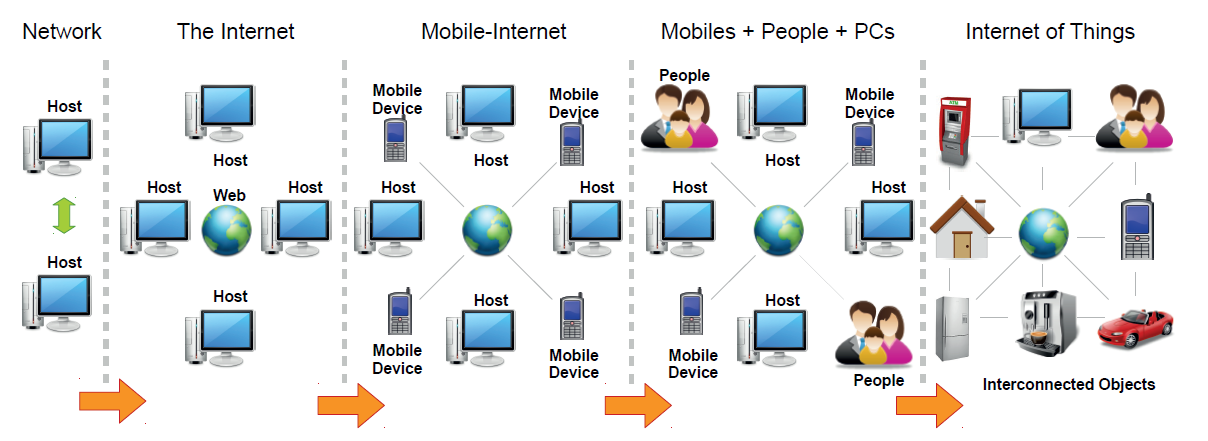
\includegraphics[width=\linewidth]{img/cap3-iot/diagrama-evolution.png}
	\caption[Evolução da internet em cinco fases]{ Evolução da internet em cinco fases (Adaptado de \cite{Our2013})}
	\label{iotEvolution}
\end{figure}



Uma das principais vantagens do IoT é a sua ligação evidente a todos os objetos, o que por si só é uma ideia avassaladora. O volume de dados gerado por este tipo de ligação pode ser interpretado pelo modelo DIKW que em inglês significa Data-Information-Knowledge-Wisdom \cite{Rowley2007}. Este modelo, também conhecido como pirâmide do conhecimento (Figura \ref{dikw}), é uma hierarquia informacional utilizada especialmente nas áreas da ciência da informação e na gestão do conhecimento, onde cada camada acrescenta certos atributos sobre a anterior.


\begin{figure}[!htb]
	\centering
	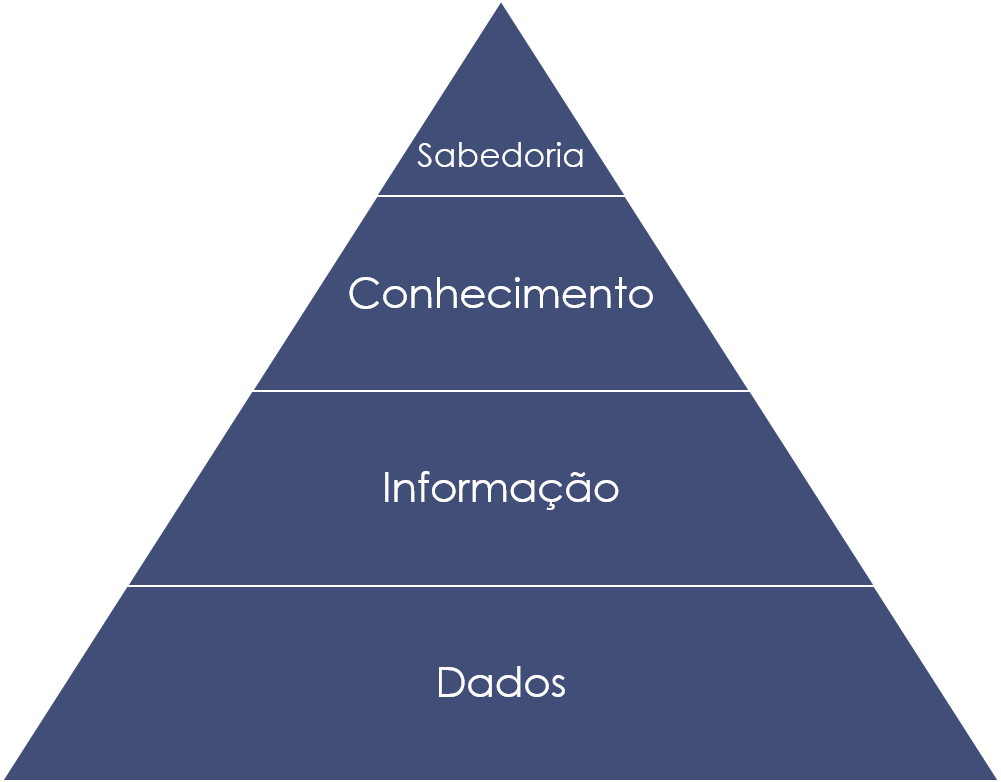
\includegraphics[scale=0.3]{img/cap3-iot/dikw.png}
	\caption{Pirâmide do conhecimento: modelo DIKW}
	\label{dikw}
\end{figure}



A ligação dos objetos à Internet acarreta benefícios visíveis à nossa sociedade, possibilitando um maior controlo e entendimento de como os sistemas interagem entre si e proporcionando uma melhor qualidade de vida a todos. Embora as vantagens se sobreponham às desvantagens não nos podemos esquecer que existem alguns problemas a nível segurança, privacidade, legislação e identidade.







\section{Considerações finais}






